\newcommand{\runTimek}{\mathcal{T}_k}
% \newcommand{\runTimesk}{\mathcal{T}_k\sp*}
\newcommand{\runTimez}{\mathcal{T}_0}
\newcommand{\scalek}{\mathcal{S}_k}
\newcommand{\Nptk}{\mathcal{N}_{{\rm point}}\sp{(k)}}
\newcommand{\Npk}{N_{{\rm proc}}\sp{(k)}}
\newcommand{\Nptz}{\mathcal{N}_{p,0}}
\newcommand{\Npz}{N_{{\rm proc}}\sp{(0)}}
\newcommand{\Nstepk}{N_{{\rm step}}\sp{(k)}}
% 
\section{Parallel performance on three dimensional interface problems}\label{sec:parallelPerformance}

In this section we present some preliminary parallel scaling results. 

For the strong scaling results we fix the grid size and solve for a fixed number
of steps on different numbers of nodes and processors.  We record the number of
time steps taken and the total CPU time used (wall clock time).  From this
information we compute $\runTimek$, the average CPU time per step for run $k$.
Let $\Npk$ denote the number of processors used in run $k$.  To measure the
parallel scaling behaviour, we define a {\em parallel scaling factor}
\[
\scalek={\runTimez\over\runTimek}~{\Npz \over \Npk}\,,
\]
which compares the CPU times per step between runs $0$ and $k$.  The run for 
$k=0$ is taken to be a reference computation with one processor. Ideally, $\scalek$ should
equal $1$ for perfect scaling. 
All calculations in this section were performed on a AMD Opteron Linux cluster with eight $2.4$GHz 
processors per node and 16 gigabytes of memory per node.

In Figure~\ref{fig:bump3dParallelScaling} we show results for solving the
three-dimensional interface problem with a Gaussian bump as described in
section~\ref{sec:scatWavy} (see figure~\ref{fig:scatBump3dFig}). The strong scaling
results are quite good for this small problem with about $5.5$ million grid points. 
By 16 processors there are not many grid points per processor and thus communication
costs become more important. 

\begin{figure}[hbt]
\begin{center}\small
%
\begin{tabular}{|c|c|c|c|c|c|c|c|} \hline
~~k~~&~ Nodes~  &~processors~&~total (s/step)~ &~init (s/step)~  &~advance (s/step)~ &  ~~$S_k$~~&  ~$S_k/S_{k-1}$~ \\ \hline
%    &          &            & s/step   & s/step   & s/step   &                \\ \hline
 0 &    1     &    1       & $4.7$    & $1.6$    & $3.1$    & ~$1.0 $~ & ~--~             \\ 
 1 &    1     &    2       & $2.5$    & $1.1$    & $1.1$    &  $.95 $  & ~$.95 $~            \\ 
 2 &    1     &    4       & $1.2$    & $.55$    & $.54$    &  $.98 $  & ~$1.0 $~            \\ 
 3 &    2     &    8       & $.72$    & $.29$    & $.35$    &  $.82 $  & ~$.84 $~            \\
 4 &    2     &   16       & $.48$    & $.18$    & $.27$    &  $.62 $  & ~$.75 $~            \\
%  5 &    2     &   16       & $.71$    & $.065$   & $.64$    &  $.63 $  & ~$.90 $~            \\
%  6 &    4     &   32       & $.39$    & $.036$   & $.36$    &  $.58 $  & ~$.92 $~            \\
%  7 &    8     &   64       & $.20$    & $.026$   & $.18$    &  $.56 $  & ~$.97 $~            \\
\hline
\end{tabular}
\caption{Strong parallel scaling for scattering from a three-dimensional interface.
The solution was solved
on grid $\Gc^{(4)}$ with approximately $5.5\times10^{6}$ grid points for $47$ steps. $S_k$ is the 
parallel scaling factor. }
\label{fig:bump3dParallelScaling}
\end{center}
\end{figure}

% 
% srun -N1 -n1 -ppdebug $cgmxp noplot bump3d -g=interfaceBump3de4.order2 -eps1=2.25 -eps2=1. -ky=5  -diss=2. tp=.1 -tf=.2 -go=go >! bump3d4N1n1.out
% 
% 
% ********* N1 n1 
% -->t=2.0000e-01 dt=4.26e-03 |div(E)|=7.94e-01 |div(E)|/|grad(E)|=3.74e-02, |grad(E)|=2.13e+01, max(u):[7.28e-01,5.92e-02,1.08e-02,]
% 
%          ---Maxwell Summary--- 
%   ==== numberOfStepsTaken =       47, grids=4, gridpts =5480036, interp pts=123356, processors=1 ==== 
%   ==== memory per-proc: [min=855.5,ave=855.5,max=855.5](Mb), max-recorded=855.457 (Mb), total=855.5 (Mb)
%    Timings:         (ave-sec/proc:)   seconds    sec/step   sec/step/pt     %     [max-s/proc] [min-s/proc]
% total time..........................  2.22e+02    4.73e+00    8.63e-07   100.000   2.223e+02   2.223e+02
% setup and initialize................  7.36e+01    1.57e+00    2.86e-07    33.127   7.364e+01   7.364e+01
% initial conditions..................  2.61e+01    5.54e-01    1.01e-07    11.720   2.605e+01   2.605e+01
% advance.............................  1.44e+02    3.06e+00    5.59e-07    64.793   1.440e+02   1.440e+02
%   advance rectangular grids.........  3.62e+01    7.71e-01    1.41e-07    16.296   3.623e+01   3.623e+01
%   advance curvilinear grids.........  1.89e+01    4.02e-01    7.34e-08     8.504   1.890e+01   1.890e+01
%    (advOpt).........................  4.16e+01    8.85e-01    1.61e-07    18.703   4.157e+01   4.157e+01
%   boundary conditions...............  4.36e+01    9.28e-01    1.69e-07    19.626   4.363e+01   4.363e+01
%   interface bc......................  1.37e+01    2.92e-01    5.33e-08     6.171   1.372e+01   1.372e+01
%   interpolation.....................  7.26e+00    1.55e-01    2.82e-08     3.268   7.265e+00   7.265e+00
%   update ghost (parallel)...........  8.99e-03    1.91e-04    3.49e-11     0.004   8.993e-03   8.993e-03
% compute dt..........................  5.07e-02    1.08e-03    1.97e-10     0.023   5.070e-02   5.070e-02
% plotting............................  2.84e+00    6.04e-02    1.10e-08     1.276   2.837e+00   2.837e+00
% 
% *********** N1 n2 
% 
%        |grad(E)|=2.13e+01 (47 steps)
% -->t=2.0000e-01 dt=4.26e-03 |div(E)|=7.94e-01 |div(E)|/|grad(E)|=3.74e-02, |grad(E)|=2.13e+01, max(u):[7.28e-01,5.92e-02,1.08e-02,]
% 
%          ---Maxwell Summary--- 
%   ==== numberOfStepsTaken =       47, grids=4, gridpts =5480036, interp pts=123356, processors=2 ==== 
%   ==== memory per-proc: [min=484.289,ave=486.41,max=488.531](Mb), max-recorded=467.477 (Mb), total=972.82 (Mb)
%    Timings:         (ave-sec/proc:)   seconds    sec/step   sec/step/pt     %     [max-s/proc] [min-s/proc]
% total time..........................  1.17e+02    2.48e+00    4.53e-07   100.000   1.167e+02   1.167e+02
% setup and initialize................  4.93e+01    1.05e+00    1.91e-07    42.214   4.927e+01   4.927e+01
% initial conditions..................  2.45e+01    5.22e-01    9.52e-08    21.015   2.455e+01   2.451e+01
% advance.............................  5.35e+01    1.14e+00    2.08e-07    45.813   5.347e+01   5.347e+01
%   advance rectangular grids.........  1.47e+01    3.14e-01    5.73e-08    12.638   1.475e+01   1.475e+01
%   advance curvilinear grids.........  9.71e+00    2.07e-01    3.77e-08     8.320   9.710e+00   9.710e+00
%    (advOpt).........................  1.79e+01    3.80e-01    6.94e-08    15.318   1.788e+01   1.788e+01
%   boundary conditions...............  2.94e+00    6.25e-02    1.14e-08     2.517   2.937e+00   2.937e+00
%   interface bc......................  7.48e+00    1.59e-01    2.90e-08     6.411   7.597e+00   7.367e+00
%   interpolation.....................  5.54e+00    1.18e-01    2.15e-08     4.743   5.588e+00   5.483e+00
%   update ghost (parallel)...........  1.04e+00    2.22e-02    4.05e-09     0.894   1.247e+00   8.401e-01
% compute dt..........................  8.33e-02    1.77e-03    3.24e-10     0.071   8.332e-02   8.332e-02
% 
% 
% ********* N1 n4 
%        |grad(E)|=2.13e+01 (47 steps)
% -->t=2.0000e-01 dt=4.26e-03 |div(E)|=7.94e-01 |div(E)|/|grad(E)|=3.74e-02, |grad(E)|=2.13e+01, max(u):[7.28e-01,5.92e-02,1.08e-02,]
% 
%          ---Maxwell Summary--- 
%   ==== numberOfStepsTaken =       47, grids=4, gridpts =5480036, interp pts=123356, processors=4 ==== 
%   ==== memory per-proc: [min=283.344,ave=287.711,max=297.531](Mb), max-recorded=297.488 (Mb), total=1150.84 (Mb)
%    Timings:         (ave-sec/proc:)   seconds    sec/step   sec/step/pt     %     [max-s/proc] [min-s/proc]
% total time..........................  5.85e+01    1.24e+00    2.27e-07   100.000   5.849e+01   5.849e+01
% setup and initialize................  2.58e+01    5.48e-01    1.00e-07    44.063   2.579e+01   2.573e+01
% initial conditions..................  1.28e+01    2.72e-01    4.96e-08    21.849   1.279e+01   1.277e+01
% advance.............................  2.55e+01    5.42e-01    9.89e-08    43.551   2.547e+01   2.547e+01
%   advance rectangular grids.........  6.56e+00    1.40e-01    2.55e-08    11.219   6.856e+00   6.175e+00
%   advance curvilinear grids.........  4.00e+00    8.52e-02    1.55e-08     6.847   4.057e+00   3.908e+00
%    (advOpt).........................  7.81e+00    1.66e-01    3.03e-08    13.356   8.058e+00   7.481e+00
%   boundary conditions...............  7.45e-01    1.58e-02    2.89e-09     1.274   7.466e-01   7.423e-01
%   interface bc......................  3.94e+00    8.39e-02    1.53e-08     6.743   4.052e+00   3.836e+00
%   interpolation.....................  3.12e+00    6.64e-02    1.21e-08     5.339   3.124e+00   3.121e+00
%   update ghost (parallel)...........  1.09e+00    2.31e-02    4.22e-09     1.859   1.284e+00   8.178e-01
% compute dt..........................  6.46e-02    1.37e-03    2.51e-10     0.110   1.089e-01   2.549e-02
% plotting............................  6.90e-01    1.47e-02    2.68e-09     1.180   6.976e-01   6.672e-01
% 


% *********************** See runs/cgmx/bump3d/memo.parallel

% interfaceBump3d1bumpe8.order2

% -->t=1.0000e-01 dt=2.44e-03 |div(E)|=1.24e-15 |div(E)|/|grad(E)|=2.54e-17, |grad(E)|=4.89e+01, max(u):[8.97e-01,8.97e-01,3.79e-26,]
% 
%          ---Maxwell Summary--- 
%   ==== numberOfStepsTaken =       41, grids=4, gridpts =41040128, interp pts=475780, processors=1 ==== 
%   ==== memory per-proc: [min=4881.86,ave=4881.86,max=4881.86](Mb), max-recorded=4881.82 (Mb), total=4881.86 (Mb)
%    Timings:         (ave-sec/proc:)   seconds    sec/step   sec/step/pt     %     [max-s/proc] [min-s/proc]
% total time..........................  1.26e+03    3.08e+01    7.49e-07   100.000   1.261e+03   1.261e+03
% setup and initialize................  1.76e+02    4.30e+00    1.05e-07    13.967   1.761e+02   1.761e+02
% initial conditions..................  1.12e+02    2.74e+00    6.68e-08     8.909   1.123e+02   1.123e+02
% advance.............................  1.03e+03    2.52e+01    6.13e-07    81.816   1.032e+03   1.032e+03
%   advance rectangular grids.........  3.85e+02    9.40e+00    2.29e-07    30.563   3.853e+02   3.853e+02
%   advance curvilinear grids.........  1.24e+02    3.01e+00    7.34e-08     9.802   1.236e+02   1.236e+02
%    (advOpt).........................  4.01e+02    9.77e+00    2.38e-07    31.784   4.007e+02   4.007e+02
%   boundary conditions...............  3.74e+02    9.12e+00    2.22e-07    29.652   3.738e+02   3.738e+02
%   interface bc......................  5.34e+01    1.30e+00    3.17e-08     4.233   5.336e+01   5.336e+01
%   interpolation.....................  9.54e+00    2.33e-01    5.67e-09     0.757   9.545e+00   9.545e+00
%   update ghost (parallel)...........  8.72e-03    2.13e-04    5.18e-12     0.001   8.720e-03   8.720e-03
% compute dt..........................  1.58e-01    3.86e-03    9.41e-11     0.013   1.583e-01   1.583e-01
% plotting............................  2.65e+01    6.46e-01    1.57e-08     2.100   2.648e+01   2.648e+01
\begin{figure}[hbt]
\begin{center}\small
%
\begin{tabular}{|c|c|c|c|c|c|c|c|} \hline
~~k~~&~ Nodes~  &~processors~&~total (s/step)~ &~init (s/step)~  &~advance (s/step)~ &  ~~$S_k$~~&  ~$S_k/S_{k-1}$~ \\ \hline
%  0 &    1     &    1       & $4.7$    & $1.6$    & $3.1$    & ~$1.0 $~ & ~--~             \\ 
 1 &    1     &    1       & $30.8$   & $4.3$    & $25.2$   &  $.   $  & ~$.   $~            \\ 
 2 &    2     &    2       & $14.1$   & $3.1$    & $9.4$    &  $    $  & ~$    $~            \\ 
 2 &    2     &    4       & $10.6$   & $2.6$    & $6.2$    &  $    $  & ~$    $~            \\ 
 3 &    2     &    8       & $5.2$    & $1.3$    & $3.0$    &  $.   $  & ~$.   $~            \\
 4 &    4     &   16       & $7.8$    & $2.2$    & $3.6$    &  $.   $  & ~$.   $~            \\
 5 &    4     &   32       & $1.3$    & $.31$    & $.78$    &  $.   $  & ~$.   $~            \\
 6 &    8     &   64       & $.79$    & $.18$    & $.49$    &  $.   $  & ~$.   $~            \\
\hline
\end{tabular}
%
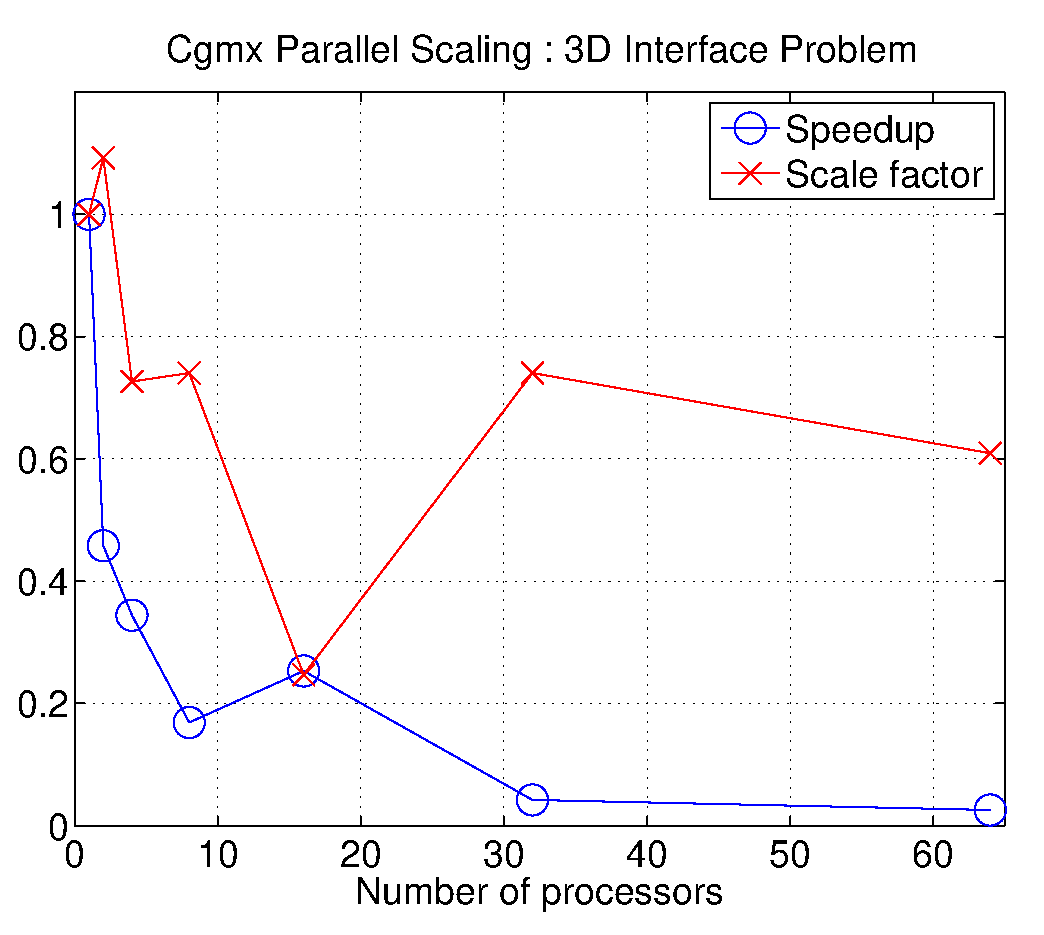
\includegraphics[width=10cm]{cgmxInterfaceParallelSpeedup.eps}
%
\caption{Strong parallel scaling for scattering from a three-dimensional interface with a bump.
The solution was solved
on grid $\Gc^{(8)}$ with approximately $41.\times10^{6}$ grid points for $41$ steps. $S_k$ is the 
parallel scaling factor. }
\label{fig:bump3dParallelScalingII}
\end{center}
\end{figure}
